%\usepackage[a4paper, margin=1in]{geometry}
\documentclass[11pt]{article}

\usepackage{glossaries}
\usepackage{graphicx}
\usepackage{titling}
\usepackage{hyperref}
\usepackage{indentfirst}
\usepackage{amsmath}
\usepackage{float}
\setlength{\parindent}{15pt}  % 들여쓰기 크기 설정 (기본: 15pt)


\makeglossaries
\newacronym{cstr}{CSTR}{Continuous Stirred Tank Reactor}
\newacronym{rl}{RL}{Reinforcement Learning}
\newacronym{dqn}{DQN}{Deep Q-Network}
\newacronym{ppo}{PPO}{Proximal Policy Optimization}
\newacronym{ddpg}{DDPG}{Deep Deterministic Policy Gradient}
\newacronym{pid}{PID}{Proportional-Integral-Derivative}
\newacronym{mpc}{MPC}{Model Predictive Control}

\begin{document}

\title{RL-Based Control of Benchmark CSTR Processes with Safety Considerations}
\author{Seunghyun Cho, Hain Lee, Jaehyun Oh}
\date{\today}


\setlength{\droptitle}{-4cm}  % 제목과 페이지 상단 간격 조정
\maketitle

\section{progress}
\subsection{CSTR \& Van de Vusse Reaction Code}


The environment code and the training code have both been implemented, yet to be connected after modification.
The environment code and the training code are mounted at \href{https://github.com/OhtoEncoder/SNU2025RL_Team16}{GitHub Repository}.

\subsection{Code Details \& Miscellaneous}

For an initial testing, we ran a reference DQN training script instead of the training code we created.
Fig \ref{fig1} shows the performance of the DQN agent in the CSTR \& Van de Vusse environment, 
illustrating that the environment is built well so that the agent is able to learn and improve its performance over time.
However, since DQN does not support multi-action or continuous action spaces,
we plan to implement a new version to support multi-action and continuous action spaces.

\begin{figure}[H]
    \centering
    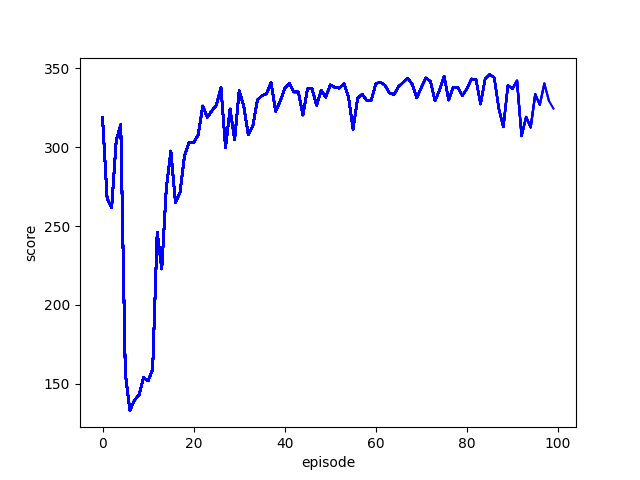
\includegraphics[width=10cm]{DQN_graph.png} % 또는 .png, .pdf 등
    \caption{Defined states and actions in previous research}
    \label{fig1}
\end{figure}

Reward shaping has not been performed yet. 
The current reward is represented in the form of a differential expression, such as $\frac{dC}{dt}$.
The simulation is set in discrete time steps.

The action space is designed to include two variables: changes in feed flow and changes in heat, 
and feed flow change is represented as a list of five discrete values: +2, +1, 0, -1, and -2. 
However, the heat component is yet to be written in code, since it is hard to implement within the DQN training code. 
This will be addressed and verified within the training code.

\begin{figure}[H]
    \centering
    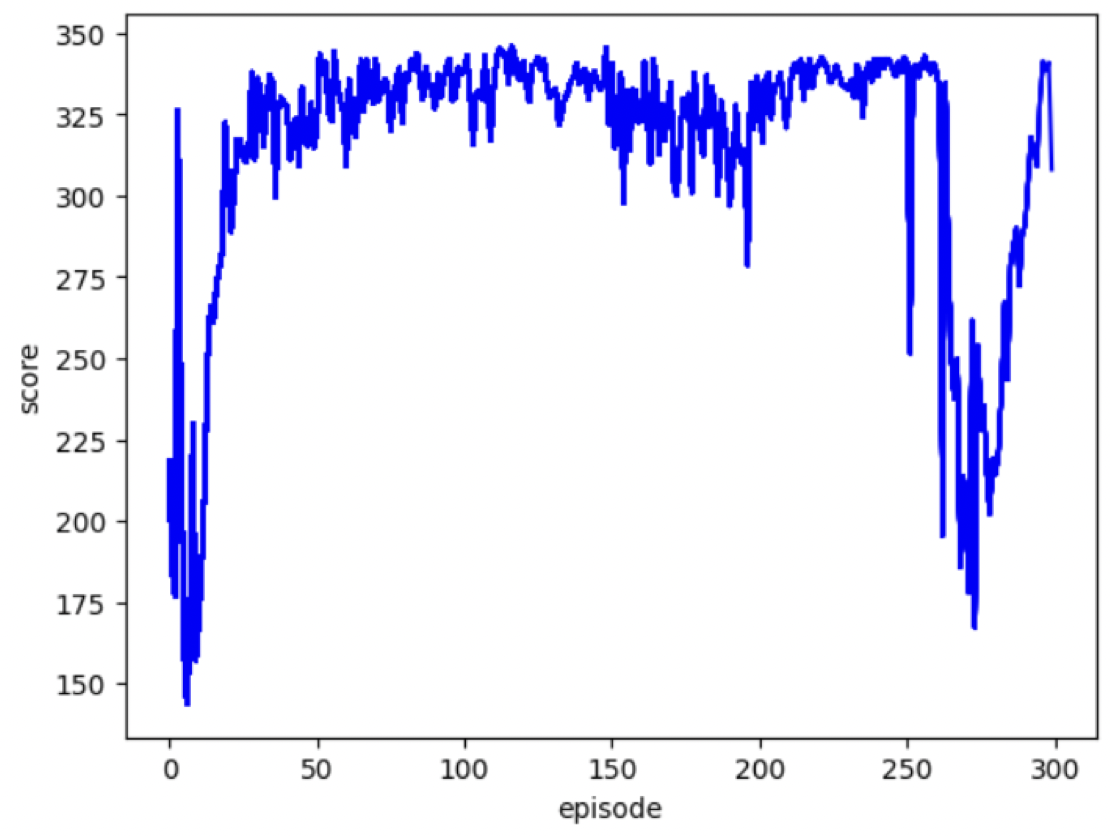
\includegraphics[width=9cm]{Fig2_buffer.png} % 또는 .png, .pdf 등
    \caption{Defined states and actions in previous research}
    \label{fig2}
\end{figure}

In Fig \ref{fig2}, we have observed that the sliding window (replay buffer) sometimes leads to a loss of important early informations, causing performance degradation in the later part of the training. 
Since the batch size is defined in terms of time steps and usually covers the entire episode, this is not a critical issue.
However, if crucial data—such as failure events—are forgotten, it could negatively affect learning.

\section{Preliminary}

The current action space is discrete, which makes it compatible with DQN.
However, DQN is inherently limited to discrete action spaces and cannot handle continuous actions.
We plan to extend the implementation to support DQN, DDPG, and PPO. 
First of all, we are considering DDPG, which supports continuous action spaces and allows for more complex, higher-dimensional actions.
PPO will be implemented, as it can accept an action array directly.
Attempting to compress multiple actions into a form compatible with DQN can lead to errors, so we aim to adopt PPO or DDPG to overcome this limitation and improve overall model flexibility.

We plan to implement reward shaping to enhance the learning process and ensure that the agent receives more informative feedback during training.
\bibliographystyle{IEEEtran}
\bibliography{references}


\end{document}


%Milestone Report [20 pts] v

%The milestone report is due May 18th. 
%The milestone report should describe progress since the proposal and the preliminary results. 
%The length should be 2-3 pages excluding the references.
%You will receive feedback from the teaching crew on the progress.

%Editable Install 방법
git clone https://github.com/MaximilianB2/pc-gym.git
cd pc-gym

pcgym/envs/benchmark/cstr.py 파일에서 reaction kinetics 수정

pip install -e .





***GPT의 타당성 검토를 꼭 받도록 하자 ***

[진행상황]
환경코드 / (학습코드 각각을 만들었고,) 아직 연결되지 않은 상태임
원래 있는 레퍼런스용 DQN 학습코드를 활용하여 돌려본 것(멀티액션, 컨티뉴어스에 쓸수있는게 없어서 만들예정)

[구체적]
리워드 사이징은 안된 상태임
(dC / dt 형식으로 작성되어있음)
time은 discrete time으로 설정되어있음

Action은 Feedflow, Heat의 두가지의 변화량으로 작성할 예정임. 
Feed flow의 변화량은 총 5개의 리스트임 (Feedflow의 변화량)+2, +1, 0, -1, -2
Heat은 dqn으로는 반영이 안되는(혹은 아직 안된) 상태 + 이 heat은 학습코드로 확인해야하는 영역


슬라이딩 윈도우(버퍼)에서 초기의 중요 정보가 망각되면서, 뒷부분의 성능이 좀 떨어지는 모습을 보이기는 함
배치의 단위는 타임스텝(어차피 한 에폭 안에 다 들어감) -> 별로 중요한건 아님
Fail에 대한 데이터처럼 중요한 정보가 망각되면...

[앞으로 할 일] - DQN, DDPG, PPO로 확장할 예정이고
액션스페이스가 discrete한데
DQN은 continuous한 액션스페이스를 못다룸(DISCRETE한 액션스페이스를 다룸)
DDPG는 continuous한 액션스페이스를 다룸, 그리고 액션개수도 늘리ㅏ고 싶어서 DDPG
PPO 를 통해 action이 array로 들어갈 수 있어서
DQN은 압축해서 넣다보니 에러가 발생가능

Safe RL: *Q-MPC* 와 N-MPC 고민중 (Reference), MPC는 기본적으로 모델을 필요로하므로...
CSTR을 위한 surrogate model을 하나 만들긴 해야함. *(근데 Nonlinearity를 다룰 수 있는지 확인필요)*

[공개용 레포지토리 하나 작성]
레포트에 업로드 예정 + 코드설명 조금 넣고